%==================================================================================

\section{ImageMagick Installation}

ImageMagick is an open-source software suite for creating, converting, modifying, and analyzing raster and vector images. At the time this work was performed, the most recent stable release available from the official ImageMagick distribution was version \texttt{7.1.2-31} \cite{imagemagick_download}.

The source code was obtained from the official ImageMagick GitHub repository and compiled using the standard configuration and installation procedure described in the ImageMagick documentation \cite{imagemagick_install_source,imagemagick_github}. The main commands used for the installation were \cite{sharma2025imagemagick}:

\begin{itemize}
    \item git clone --depth 1 --branch 7.1.2-31 \url{https://github.com/ImageMagick/ImageMagick.git} ImageMagick-7.1.2-31
    \item cd ImageMagick-7.1.2-31
    \item ./configure
    \item make
    \item sudo make install
    \item sudo ldconfig
\end{itemize}

After the installation, the installed version was verified using: magick -version

\begin{figure}[H]
    \centering
    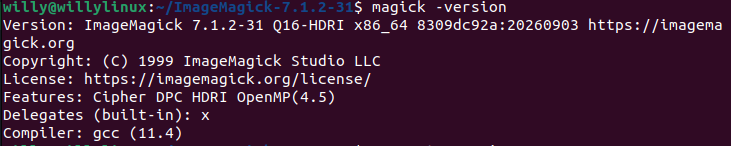
\includegraphics[width=0.9\linewidth]{assets/magick_version.png}
    \caption{Verification of the installed ImageMagick version.}
\label{fig:imagemagick-version}
\end{figure}

Several command-line operations were performed in order to become familiar with the main ImageMagick functionalities. First, an example image was generated using one of the images included with ImageMagick:

\begin{verbatim} magick logo: original.png \end{verbatim}

Information about the image, such as its dimensions, format, color space, and bit depth, can be obtained with the \texttt{identify} command:

\begin{verbatim} magick identify original.png \end{verbatim}

\begin{figure}[H]
    \centering
    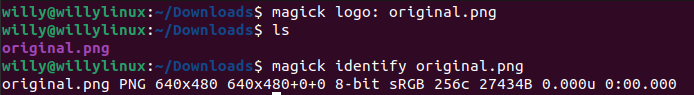
\includegraphics[width=0.9\linewidth]{assets/basic1.png}
    \caption{Basic commands 1.}
    \label{fig:commands1}
\end{figure}

ImageMagick can then apply a wide variety of transformations. Some of the operations tested were resizing, rotation, grayscale conversion, cropping, and blurring:

\begin{verbatim}
magick <input> -resize 50% <output>
magick <input> -rotate 20 <output>
magick <input> -colorspace Gray <output>
magick <input> -crop 300x200+20+20 <output>
magick <input> -blur 0x3 <output>
\end{verbatim}

\begin{figure}[H]
    \centering
    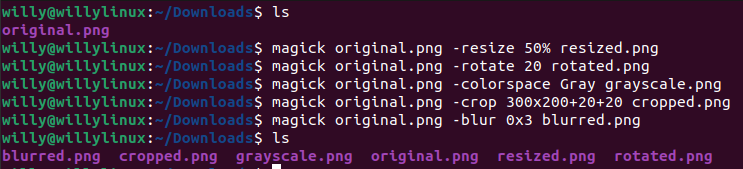
\includegraphics[width=0.9\linewidth]{assets/basic2.png}
    \caption{Basic commands 2.}
    \label{fig:commands2}
\end{figure}

\begin{figure}[H]
    \centering
    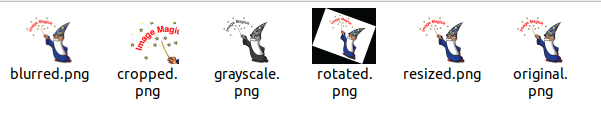
\includegraphics[width=0.9\linewidth]{assets/images_example.png}
    \caption{Example of the images created.}
    \label{fig:exampleimages}
\end{figure}

Figure~\ref{fig:exampleimages} shows the results of these operations. These experiments illustrate that ImageMagick can be used not only for format conversion but also for image transformations, color-space manipulation, filtering, image composition, and image inspection.

The formats supported by the installed version can be inspected with:

\begin{verbatim} magick identify -list format \end{verbatim}

In particular, the output contains the \texttt{AVS} format identified as \emph{AVS X image}, with both reading and writing support \cite{imagemagick_formats}.

\begin{figure}[H]
    \centering
    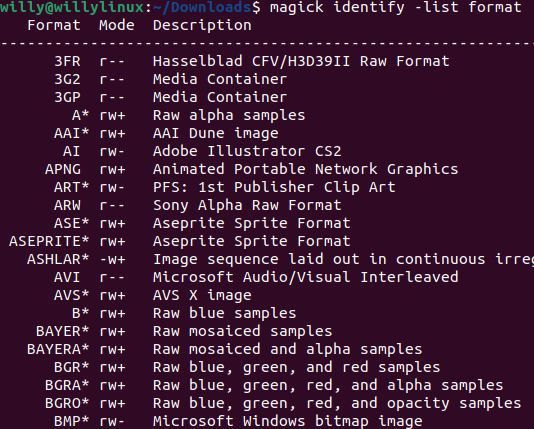
\includegraphics[width=0.7\linewidth]{assets/formats.png}
    \caption{Example of some formats in Image Magick.}
    \label{fig:imagemagick_formats}
\end{figure}

%==================================================================================

\section{ImageMagick: AVS Format}

ImageMagick identifies the \texttt{AVS} format as the \emph{AVS X image} format and provides both reading and writing support for it \cite{imagemagick_formats}. The format should not be confused with video formats that use the same AVS acronym.

The AVS X-Image format originated on UNIX workstations and was commonly used to represent true-color raster images with transparency information. Each pixel contains four 8-bit components, giving a total of 32 bits, or four bytes, per pixel \cite{goldensoftware_avs}. The four components are stored in the order alpha, red, green, and blue (A-R-G-B) \cite{bourke_avs,imagemagick_avs_source}.

The internal structure of a single AVS X-Image is particularly simple. The file begins with an 8-byte header followed immediately by the raster pixel data \cite{bourke_avs}. The header contains two unsigned 32-bit integers representing the image width and height. Both integers are stored using most-significant-byte-first, or big-endian, byte ordering \cite{imagemagick_avs_source}.

Pixels are stored from left to right and from the top of the image to the bottom \cite{bourke_avs}. For each pixel, one unsigned byte is stored for each of the four components: a == alpha, r == red, g = reen, b == blue, where each colour/alpha component is 1 unsigned byte \cite{bourke_avs}.

Unlike formats such as PNG or JPEG, the basic AVS X-Image representation does not contain a complex metadata structure or compressed image stream. ImageMagick's AVS encoder writes the width (the first four bytes) and height (the next four bytes) directly, followed by the four channel bytes for every pixel \cite{imagemagick_avs_source}.

For example, to verify the internal structure of the AVS format, the image show next will be converted from JPEG to AVS using ImageMagick.

\begin{figure}[H]
    \centering
    
\includegraphics[width=0.35\linewidth]{assets/smiley.jpg}
    \caption{Original image used for the AVS format experiment.}
    \label{fig:smiley-original}
\end{figure}

The image can be converted to .avs using:
\begin{verbatim} magick smiley.jpg smiley.avs \end{verbatim}

\begin{figure}[H]
    \centering
    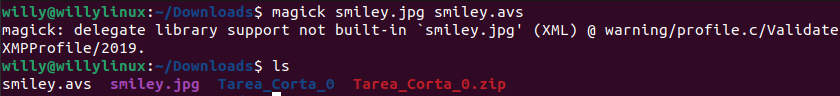
\includegraphics[width=0.9\linewidth]{assets/smiley_converted.png}
    \caption{Image in .avs format.}
    \label{fig:smiley-original}
\end{figure}

The original image has a resolution of $612 \times 612$ pixels. The first bytes of the resulting AVS file can be examined with:

\begin{verbatim} xxd -g 1 -l 32 smiley.avs \end{verbatim}

Since 612 in hexadecimal is \texttt{0x264}, its 32-bit big-endian
representation is 00 00 02 64. Therefore, the first eight bytes of the AVS file are: 00 00 02 64  00 00 02 64.

\begin{figure}[H]
    \centering
    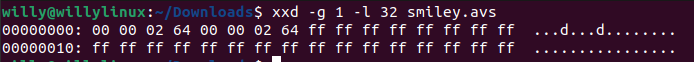
\includegraphics[width=0.9\linewidth]{assets/smiley_stats.png}
    \caption{Bytes in a .avs format.}
    \label{fig:smiley-original}
\end{figure}

As a matter of fact, the term AVS is also associated with scientific-visualization formats that should not be confused with AVS X-Image. In particular, AVS Field files, commonly identified by the \texttt{.fld} extension, are designed to describe multidimensional scientific datasets rather than ordinary two-dimensional raster images.

Scientific-visualization research such as the work of Nonaka et al. discusses visualization of large-scale datasets on high-performance computing systems \cite{nonaka2018sparc64fx}. Such scientific data representations serve a different purpose from the AVS X-Image format implemented by ImageMagick.